\documentclass[12pt]{article}

\usepackage{graphicx}
\usepackage[hidelinks]{hyperref}
\usepackage{color}
\usepackage[utf8x]{inputenc}
\usepackage{ucs}
\usepackage[spanish]{babel}
\usepackage{amsmath}
\usepackage{amsfonts}
\usepackage{amssymb}
\usepackage{makeidx}
\usepackage[hidelinks]{hyperref}
\usepackage[left=2cm,right=2cm,top=2cm,bottom=2cm]{geometry}

\title{\textbf{Circuitos de Control de Voltaje y Corriente con Tiristores}}
\author{R\\ Jes\'us David Esparza Cabrera\\
		Sistemas Electronicos de Interfaz\\Ing. Mecatr\'onica\\Mtro. Carlos Enrique Mor\'an Garabito\\
		Viernes, 1 de Noviembre 2019}
\date{}


\begin{document}
\maketitle
\begin{figure}[htp]
\centering

\includegraphics[scale=1.5]{/media/david/HOLA JAJA/EV.1.3/LOGO.png}
\label{}
\end{figure}

\pagebreak

\section{Introducci\'on}

El Dimmer es un control de iluminaci\'on que tiene como funci\'on controlar la intensidad de iluminaci\'on de una lampara, no es otra cosa, que la principal funci\'on de esta practica.

Para esta practica el circuito conformado  por pocos componentes, en el cual el m\'as relevante es el Triac, ya que est\'e, al recibir en su pin conocido como gate, la descarga de el Diac, este permite que el Triac pueda circular la corriente a trav\'es de sus terminales para alimemtar a la carga, funcionando como un interruptor.\\ 
  Tipos de Dimmers:
 - Dimmer para lámparas incandescentes (utilizado en el voltaje normal de 230 V). Se pueden regular con dimmer pero están condenadas a desaparecer.

 - Dimmer para lámparas halógenas (dos clases a una tensión de 230 V y una tensión en el intervalo de 10 a 24 V)

 - Dimmer para lámparas fluorescentes y luces fluorescentes compactas CFL. Las lámparas fluorescentes normales no se pueden regular, las CFL si llevan la etiqueta de regulable si se podrá regular con un dimmer.

 - Dimmer LED para bombillas LED que es la tecnología más avanzada. La eficiencia energética está impulsando a los consumidores a reemplazar las lámparas incandescentes estándar por lámparas LED y serán las que utilizaremos casi en exclusiva, por este motivo luego los veremos con más detalle.

 Cuando tengamos claro el tipo de lámpara que tenemos o vamos a comprar podemos elegir el dimmer adecuado.

 Dese el punto de vista de como se regula la luz tenemos 2 tipos diferentes:

 - Dimmer con selector: tienen una rueda que al girarla se regula el nivel de luz. Este es el tipo recomendado si la instalación es nueva.


\begin{figure}[htp]
\centering
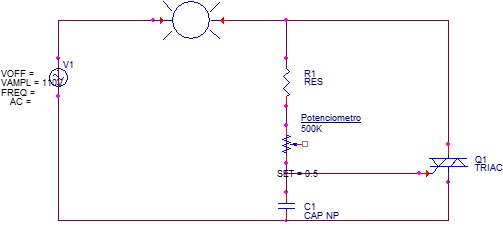
\includegraphics[scale=1.00]{/media/david/HOLA JAJA/EV.1.3/CIRCUITO.jpg}
\caption{Circuito}
\label{}
\end{figure}

\textbf{Conclusiones}\\
Jes\'us David Esparza Cabrera.\\
En este circuito me permitio de manera muy sencilla el funcionamiento de un Dimmer, en el cual me pude percatar de la gran inportancia del triac para esta ocaci\'on, ya que este funciona o puede funcionar como un atenuador de focos incandecentes y como un regulador de velocidad, lo que me permitio conocer y aprender el funcinamiento de este mismo.

\end{document}